\documentclass[final]{ukthesis}
%you must include these 2 packages.
\usepackage{amsmath}
\usepackage[pdfauthor={Jack Bandy},
            pdftitle={The Title},
            pdfsubject={The Subject},
            pdfkeywords={Some Keywords},
            pdfproducer={Latex with hyperref},
            pdfcreator={latex->dvips->ps2pdf},
            pdfpagemode=UseOutlines,
            bookmarksopen=true,
            letterpaper,
            bookmarksnumbered=true]{hyperref}
\usepackage{memhfixc}
\usepackage{graphicx}
\graphicspath{{./figures/}}
%%%%%%%%%%%%%%%%%%%%%%%%%%%%%%%%%%%%%%%%%%%%%%%%
\begin{document}
%author data
\author{Jack Bandy}
\title{INTERACTIVE MACHINE LEARNING FOR WORD RECOGNITION ON DAMAGED HANDWRITTEN DOCUMENTS}
\abstract{an abstract}
\advisor{Brent Seales}
\keywords{keywords go here}
\dgs{Miroslaw Truszczynski}
%the title pages
\frontmatter
\maketitle
\begin{acknowledgments}
Acknowledge people/things here
\end{acknowledgments}
\tableofcontents\clearpage
\listoffigures\clearpage
\listoftables\clearpage
%----------------------------------------------
\mainmatter


%%
%
%
% Introduction Chapter
%
%%
\chapter{Introduction}

This project deals with automated word recognition for historical documents, especially documents that have been physically damaged.

Extensive research exists in printed text recognition and handwriting recognition, and for modern data, the input to these problems is remarkably clean. Historical data, such as that considered in this project, presents challenges that are not often considered in related literature. For example, although many projects for handwritten word recognition consider variations caused by penmanship, very few consider variations caused by physical damage.

This chapter reviews related literature, motivates an alternative approach, and outlines the contributions of the project.

%
% Related Work
%
\section{Related Work}
For several decades, researchers have been developing methods for automated character and word recognition. These methods take some photograph(s) of printed or handwritten text as input, and produce a transcript of that text as output. This section provides a brief summary of methods which have influenced the course of this research area, including advances in handwriting recognition, printed text recognition, and handwritten word spotting.

The nomenclature for these related tasks can be somewhat inconsistent in the literature. For the purposes of this paper, ``handwriting recognition'' differs from ``handwritten word spotting'' in that the former aims to create full transcriptions while the latter merely locates and/or recognizes instances of a given word within a document. ``Printed text recognition,'' although it uses many of the same methods, refers to projects that examine machine-printed texts. As detailed in the following sections, the fields have essentially converged at this point, but a distinction is necessary for the previous decades.


% Text Recognition Subsection
\subsection{Text Recognition}
From a technical standpoint, automatic text recognition is the task of turning an image into the text within the image. ``Text recognition'' here refers to recognizing {\em printed} texts, not handwritten texts, which prompts several convenient assumptions. Namely, that all occurrences of a given character will be nearly identical in shape and size. Because of this assumption, researchers could attempt letter-for-letter recognition on documents, a process known as object character recognition (OCR).

OCR on scans of printed documents has seen success since as early as the 1980s \cite{mantas1986overview,govindan1990character}, with methods detailed as early as the 1950s \cite{glauberman1956character}. A survey from 1996 \cite{trier1996feature} notes that, due to the consistency of letter shapes and sizes in question, simple techniques such as projection histograms, template matching, zoning, and geometric moments were successful. As early as 1987, font and size constraints were no longer needed. The authors of \cite{kahan1987recognition} demonstrated a system that accurately classified mixtures of dissimilar fonts of varied sizes.

Gradually, more and more constraints were eliminated. After \cite{kahan1987recognition} removed the need for font and size assumptions, the race was on to eliminate constraints such as alignment, color, contrast, and more. Eventually, the task of printed text recognition was one that could be done ``in the wild,'' \cite{smith2007overview,wang2012end,jaderberg2016reading} with essentially no assumptions about the nature of the text. Especially important for ``in the wild'' recognition was eliminating the segmentation step, as in \cite{rusinol2015efficient}, such that regions of text could be found without a processing phase devoted to localization. The ideal system, then, would be able to recognize text in any image in which a human could see text.

An important benchmark dataset for this kind of text recognition is Street View Text (SVT) \cite{wang2010word}. SVT was harvested using pictures from Google Street View, and thus contains a heterogeneous collection of word images with a variety of fonts, colors, and backgrounds. (Despite the variations, word images in this set do not include handwritten characters.) The SVT dataset was released in 2010, and by 2012, \cite{wang2012end} used it to train a neural network that achieved state-of-the-art performance for both character recognition and word recognition. The high degree of accuracy was achieved via unsupervised feature learning and convolutional neural networks.

In fact, even before 2012, many researchers realized that convolutions were ideal for recognizing the shapes of different letters and words \cite{saidane2007automatic,delakis2008text}, and the trend only became stronger after successes like \cite{wang2012end}. Convolutional neural networks (CNNs) offered exceptional performance with lower computational costs than ``fully-connected'' neural networks. Today, many robust approaches to text recognition exist via CNNs \cite{wang2012end,yin2014robust,jaderberg2016reading}.


% Handwriting Recognition Subsection
\subsection{Handwriting Recognition}
Although modern methods for printed text recognition overlap methods for handwriting recognition, especially with CNNs for ``in-the-wild" recognition, the convergence happened after years of parallel research. Handwriting recognition can be divided into two major categories, ``online" handwriting recognition and ``offline" handwriting recognition. In the former, software tracks the location of a writing utensil as a user moves it across some surface to produce letters and words, and the precise location and motion of the utensil helps reveal the intended writing. For example, UNIPEN \cite{guyon1994unipen}, a benchmark dataset for online handwriting recognition, includes ``pen trajectory" data that specifies when and where the pen touched down and lifted up, as well as the coordinates for the path of the pen.

More relevant to this project is the task of {\em offline} handwriting recognition, in which the input comprises only a picture of the handwriting and no additional information about its creation. A canonical example of the text recognition task is the MNIST dataset \cite{lecun1998mnist}. MNIST comprises grayscale images of individual handwritten digits, 0 to 9, and the objective is to classify each image into the digit written inside of it. Machine learning researchers have been using this task as a benchmark for several decades \cite{bottou1994comparison}, with error rates well below 1\% since 2003 \cite{kussul2004improved}.

Projects using MNIST and similar datasets are premised upon many constraints, although they differ from those made for printed text. Rather than assuming consistency in size and shape, the projects assume a very small vocabulary or character set, which can be accurately recognized with properly alignment and segmentation. As soon as a text ventured outside those constraints (misspelled words, new characters, etc.), the system would falter. Even moderately successful recognition on unconstrained datasets did not exist until the early 2000s.

This changed with the use of hidden Markov Models (HMMs) \cite{marti2001using,bunke2004offline,el1999hmm}. HMMs utilized statistical models built for specific languages to narrow down the classifications for a given letterform. A common example in english is that when a ``q'' occurs, a well-trained HMM will know to expect a ``u'' to follow. With HMMs, character and word recognition accuracies improved to over 85\% (varying with respect to the test corpus) on ``unconstrained" texts.

Although the texts were nominally unconstrained datasets, many demonstrations were still using the IAM dataset \cite{marti2002iam}, an ad-hoc database for researchers. In other words, {\em truly} unrestricted handwriting recognition was still a long way off even after the strides made by HMMs. Moving forward, a collection of George Washington letters became the de-facto standard. This dataset comprises hundreds of manuscript pages from the Library of Congress, handwritten by George Washington's secretaries. (A subset of this dataset is used in the evaluation portion of this project.)

In the mid-2000s, state-of-the-art HMM methods yielded word error rates around 50\% on {\em truly} unrestricted datasets such as the George Washington collection. But around this time, researchers began taking a new angle at the problem. Specifically, projects focused on the process of ``handwriting retrieval,'' rather than attempting complete transcriptions. Such projects allow users to query a dataset of images for a given word, and essentially scans the images for visual matches of that word. For example, \cite{rath2004search} presents a retrieval system that achieves 63\% mean average precision scores on the George Washington collection.

In \cite{rath2007word}, the word retrieval approach is formalized as a viable way to generate a searchable index of handwritten papers. Their method of ``wordspotting'' turns the search problem into a clustering problem, where word images that are ``closest'' to the query word are considered matches. Wordspotting is considered more thoroughly in the following section, however it is crucial to note that this approach eliminated the need for recognizing words before retrieval. In other words, rather than generating a full index beforehand, matching is done in real-time.

Building upon the success of wordspotting techniques and HMMs, \cite{howe2009finding} takes a step further and first detects handwritten {\em characters} in a word, then infers a word using an ensemble of HMMs. This approach allowed the recognition of words that were never seen during training, and established new standards for the George Washington dataset.

By the time ensemble HMMs came onto the scene, neural networks were already penetrating the field of handwriting recognition \cite{fernandez2007application}. By 2010, advanced techniques such as bidirectional long short-term memory (BLSTM) were successfully applied to wordspotting \cite{wang2010word} and outperformed other methods. Finally, recurrent neural networks \cite{frinken2012novel} eliminated the need for word segmentation in addition to improving state-of-the-art performance on recognition tasks.

More recently, convolutional neural networks (CNNs) have become the state-of-the-art approach for text recognition on handwritten documents \cite{zhong2016spottingnet,sudholt2016phocnet}. Many of these approaches overlap text recognition methods mentioned in the previous section, and in fact, recent neural networks are designed to recognize both printed text and handwritten text.

% Highly relavant stuff
\subsection{Word Spotting on Damaged Handwritten Documents}
In this section, the scope of related projects is narrowed down from all handwriting recognition systems, and I examine research related to word spotting on historical documents.

As previously mentioned, \cite{rath2007word} formalized the idea of wordspotting. However, the concept was originally proposed in \cite{manmatha1996word}, which clustered similar words to be annotated by users, and reported success for single-author documents with high-quality scans of the handwriting. \cite{tomai2002transcript} acknowledges some of the main challenges for historical documents: perfect line and word segmentation is nearly impossible, and unconstrained word recognition is extremely difficult. Although their proposed ``transcript mapping" method assumes a pre-existing transcript for the input image, it introduces concepts for handling variable baseline position, line skew, character size, and inter-line distance.

A fairly complete system for retrieving words in handwritten manuscripts is presented in \cite{rath2004search}. Once again, the solution steers away from the challenging task of full-on handwriting {\em recognition}, and instead focuses on retrieval of individual words. The goal is to provide a way for users to search the document, not necessarily to reveal its exact contents.

After performance improved on retrieval, around 2009, researchers began returning to the recognition task. A segmentation-free approach described in \cite{howe2009finding} utilizes character detection to improve state-of-the art performance on the GW20 manuscript. Because it is character-based, their system also recognizes words not seen in the training phase, the first such achievement for handwritten cursive manuscripts.


The Parzival database \cite{fischer2010ground}, a medieval German text from the 13th century, became a popular evaluation benchmark, and \cite{fischer2014combined} used it to demonstrate a system for full-on recognition, although it relied on a predetermined vocabulary. The following year, \cite{rusinol2015efficient} match state-of-the-art performance with a segmentation-free approach to word spotting, and by 2016, as they had done for printed text recognition and handwriting recognition, CNNs had set new standards for word spotting in historical documents \cite{sudholt2016phocnet,zhong2016spottingnet,krishnan2016deep} .


Finally, several projects have explored the interactive approach to word annotation. A familiar example is ReCAPTCHA \cite{von2008recaptcha}, a system which methodically crops pictures of book pages into images of individual words, then, using many different users to label individual word images, it produces a full transcript of the page and the book. To extend this method to take advantage of machine learning techniques, \cite{biller2013webgt} demonstrates a similar system for generating ground truth for any dataset. Like ReCAPTCHA, it allows users to annotate manuscript excerpts with labels for characters and words. However, the goal of the system is to create training data for an ML-based word recognition or word spotting system.


%
% Motivation
%
\section{Motivation}
From the review of related work, printed text recognition, handwritten word recognition, and handwritten word spotting may appear to be solved problems. The explosion of machine learning research ? in particular convolutional neural networks ? has led to drastic improvements in performance on these tasks, and many advancements have even found their way to consumer products. For example, default software on most PCs allows users to search within scans or photographs of printed typeface, and note-taking software can now interpret penmanship that would be indecipherable to many human readers.

However, the process of automatically transcribing damaged documents presents a niche area of text recognition which is not addressed well by standard approaches. Many historical documents, including those reviewed in this project, were meticulously transcribed with legibility comparable to typeface, suggesting that automated transcription would be straightforward. But over time, these documents have incurred damage of all different kinds. The characters originally may have looked like typeface, but after hundreds of years of human handling, physical corrosion, chemical decay, and other processes, reading certain parts of these documents is an arduous task even for skilled textual analysts. For such cases, neither fully human transcription nor fully automated transcription is ideal.

While fully manual transcription is the most accurate solution, it is incredibly time-consuming for larger documents. Moreover, on damaged documents, skilled papyrologists are required to decipher texts. This makes human transcription prohibitively costly in terms of time and skilled personnel.

A fully automated transcription algorithm may successfully transcribe certain portions of a historical document, but the damaged portions can distort the algorithm's output to the point of being unusable. This is especially true in cases where letters are literally missing, since OCR algorithms often assume constant width and spacing within a document.

An ideal solution would leverage automated transcription for the undamaged portions, and allow a human reader to fill in any gaps. Figure \ref{hcml-schematic} shows the potential architecture of such framework, which was presented in \cite{schaekermann2016resolvable}, which also provides an elegant schematic of the approach in Figure \ref{fig:hcml-schematic}.


\begin{figure}[t]
\begin{center}
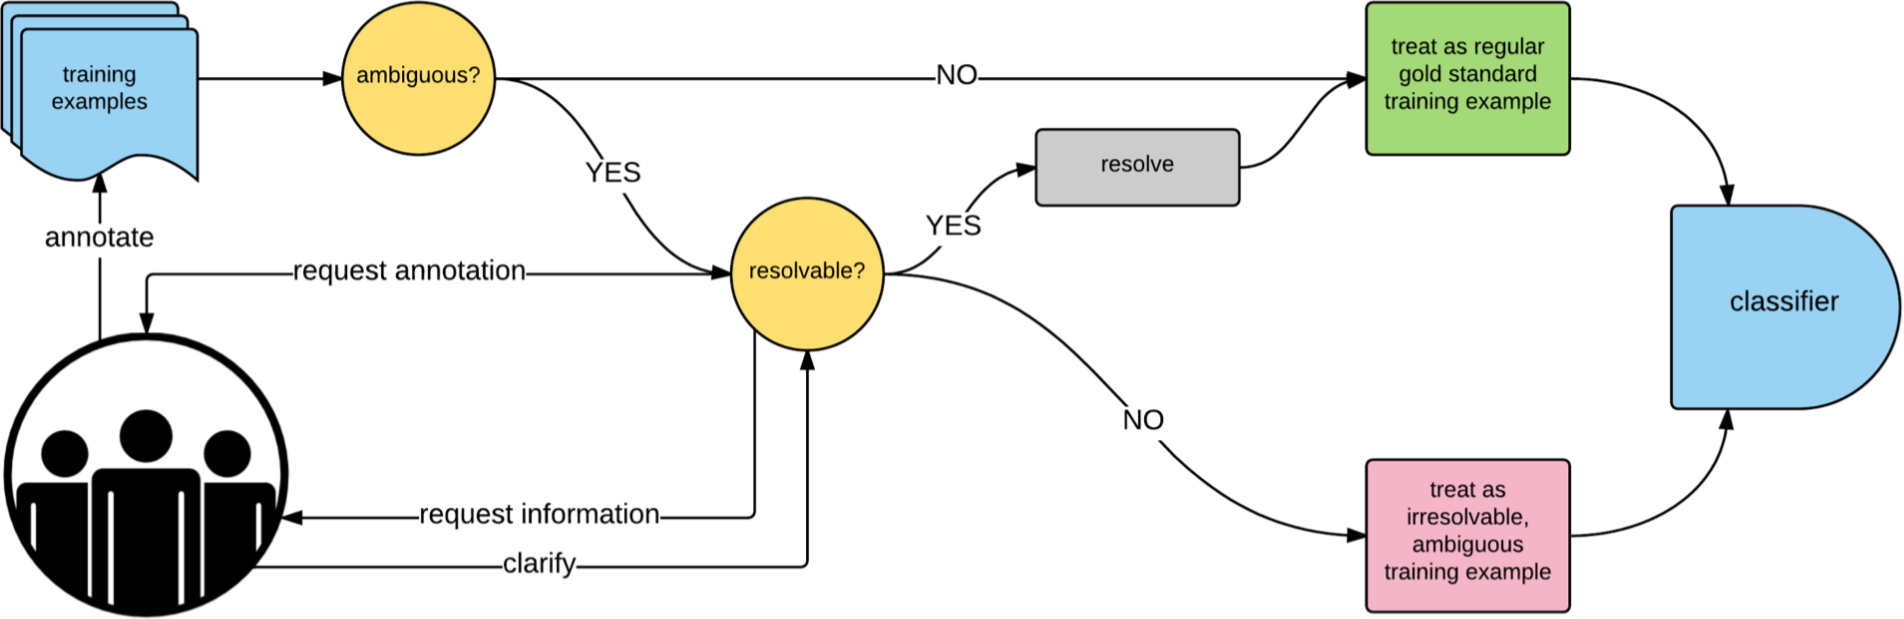
\includegraphics[width=14cm]{hcml-schematic}
\end{center}
\caption{A schematic diagram from \cite{schaekermann2016resolvable} for semi-automated transcription, designed especially for resolving ambiguity. Although resolving ambiguity is not the focus of my project, this diagram depicts a collaborative framework between machine learning and human annotation.}
\label{fig:hcml-schematic}
\end{figure}

I refer to this as semi-automated transcription. This project presents a pipeline for semi-automated transcription, blending the irreplicable abilities of the human eye with the efficiency and scalability of character recognition algorithms.



%
% Motivation
%
\section{Contributions}
The methods used in this project borrow heavily from methods in the aforementioned research areas, including keyword and character spotting \cite{sharma2015adapting,frinken2012novel}, word recognition \cite{howe2009finding}, and handwriting recognition \cite{fischer2013fast,bluche2013feature}.

Nonetheless, the project makes two notable contributions to the area of handwritten text recognition, both concerned with the challenges of damaged words. First, a framework for semi-automated transcription is detailed and implemented, in which damaged words could be labeled by an expert and seamlessly integrated into an otherwise automated word spotting process. The second contribution is an approach for virtually restoring damaged or low-quality words into a representation that could be recognized automatically.


\subsection{An Interactive Approach to Word Spotting}
A semi-automated approach to word spotting utilizes user-provided labels of words in a given document. Essentially, the system allows users to label an image, and then uses that label to annotate similar word images. This essentially lets the user label a cluster of images, while still allowing a user to correct an incorrect classification from the clustering algorithm.

There are several benefits to this semi-automated system which will be discussed in later sections.


\subsection{A Technique for Virtual Ink Restoration}
To deal with the problem of damaged and distorted words, this project presents a variational autoencoder (VAE) for restoring words with missing letters or partial letters. As long as an undamaged occurrence of the word exists somewhere in the training set, the VAE can capture and recreate the word's appearance. Not only does the recreation lead to accuracy improvements for automated recognition, it also allows users to view an enhanced version of the damaged manuscript.




%%
%
%
% Methodology Chapter
%
%%
\chapter{Methodology}


%
% Motivation
%
\section{Preprocessing}
For the George Washington and Parzival datasets, segmented and binarized word images are already provided courtesy of \cite{fischer2012lexicon}. For the Wycliffe dataset, several preprocessing steps must be taken to get from raw images of the manuscript to segmented, binarized word images suitable for word spotting. 

\subsection{Alignment}

\begin{figure}[t]
\begin{center}
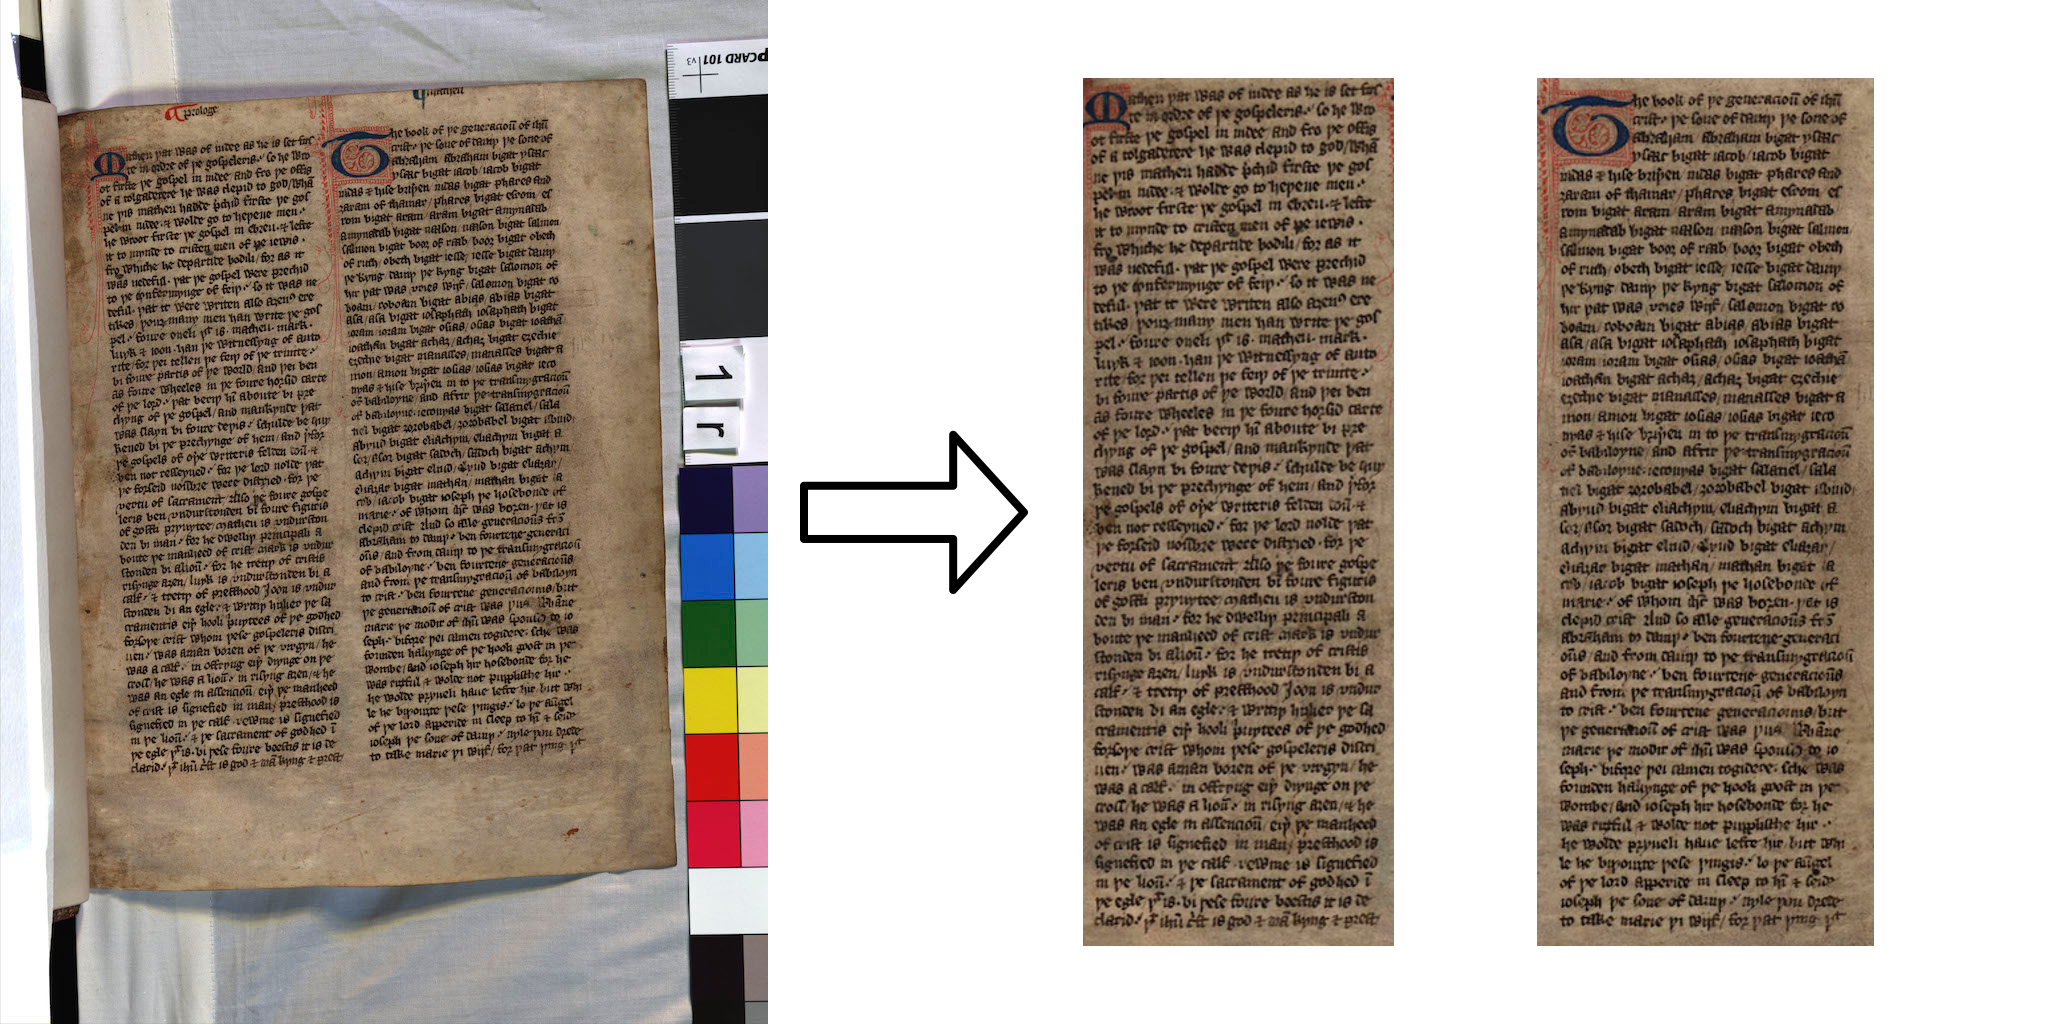
\includegraphics[width=14cm]{rotate-crop}
\end{center}
\caption{A sample of the original photographs of the Wycliffe New Testament Manuscript. In the preprocessing phase, these images must be aligned and cropped into separate columns.}
\label{fig:rotate-crop}
\end{figure}
The first step, visualized in figure \ref{fig:rotate-crop}, involves rotating the original photographs so that text columns are vertically aligned. Rotation varies depending on where the page existed in the binding and which side of the book it was on.

Columns were cropped identically on each page, based on the assumption that more precise cropping would take place in the line segmentation and word segmentation algorithms. The key in column cropping is to create images that are vertically aligned and only contain text from one column. The amount of margin outside the column need not be precise, however, to allow for key assumptions in the binarization phase, it must not contain anything besides paper.


\subsection{Binarization}
Once the column images are cropped, the RGB image is flattened into a single grayscale channel. The image is then inverted so that the text is white and the background dark gray. Next, the image is thresholded to create a binarized representation. Because lighting and coloring varies across manuscript pages, a simple global threshold would lead to noisy and inconsistent background removal. Instead, a threshold should be calculated individually for each page. This is simply referred to as ``adaptive thresholding,'' and considering the nature of the data leads to a natural choice of algorithm for this process.

Because the column image is assumed to only contain ink and paper, a histogram of values in the column image should be bimodal (the two peaks representing the approximate value of an ink pixel and a paper pixel). To remove the paper background pixels, the system uses Otsu's thresholding algorithm \cite{otsu1979threshold} as implemented by OpenCV \cite{bradski2000opencv}. Otsu's binarization algorithm takes advantage of the bimodal distribution. It works by choosing a threshold value in between the two peaks that minimizes the variance within the two ``classes,'' an ideal method for these manuscript pages.


\subsection{Line Segmentation}
After column images are binarized, the next step is to split the column into its individual lines and words.

The Wycliffe New Testament is aligned and spaced with remarkable consistency, and the segmentation technique takes advantage of this. A vertical projection profile of a binarized page image is used to determine the approximate location of individual lines of text, because the relative minimum values of the profile correspond to the spaces in between lines of text. This is visualized in Figure \ref{projection-profile-lines}.

\begin{figure}[h]
\begin{center}
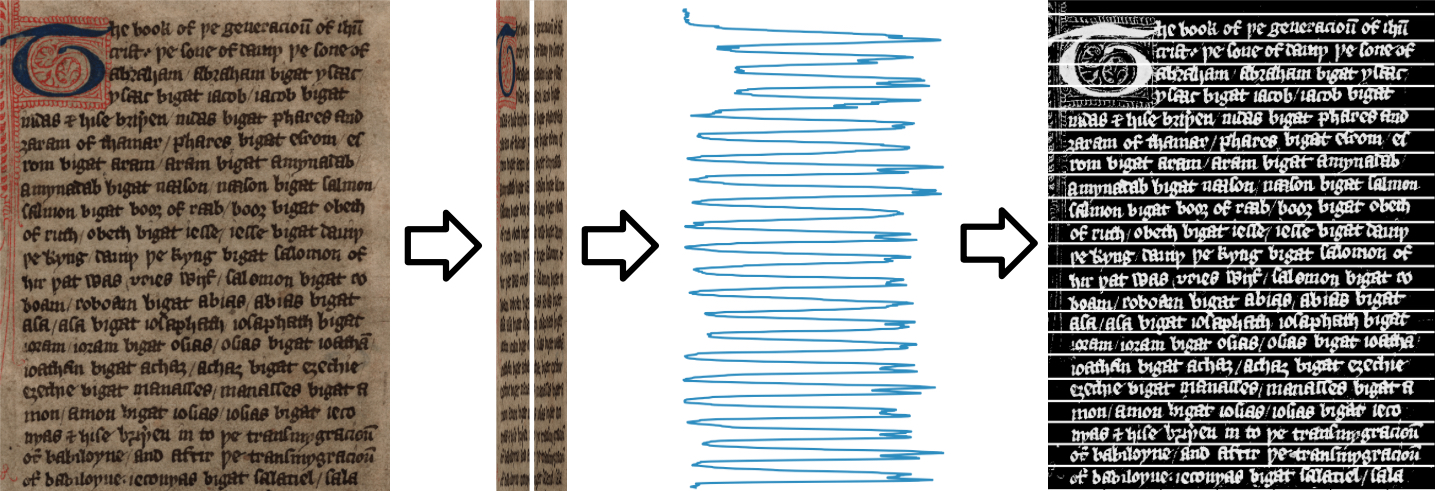
\includegraphics[width=10cm]{projection-profile-lines}
\end{center}
\caption{The projection profile used to segment lines of text. To generate words, an identical process}
\label{fig:projection-profile-lines}
\end{figure}

However, because lines are relatively wide (10-12 words), writing on some pages is slightly slanted. Figure \ref{fig:flat-vs-tilted} illustrates the dilemma of horizontal segmentations.

To segment tilted lines of text, a line of best fit must be generated across the words. This is achieved by taking the coordinates of all the nonzero values (i.e. values above the ink threshold) in the approximated horizontal text region, and applying random sample consensus (RANSAC) \cite{fischler1987random} to generate a line that fits the overall tilt of the given line. The resulting approximation eliminates most word cutoff.

\begin{figure}[t]
\begin{center}
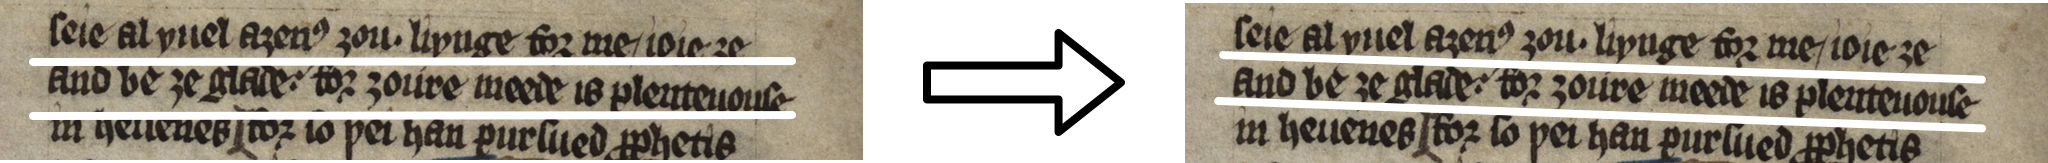
\includegraphics[width=8cm]{flat-vs-tilted}
\end{center}
\caption{Illustrating the need for tilt during the line segmentation phase. Although the column has been aligned vertically, perfectly horizontal approximations (above) for line segmentation result in cutoff words. Tilted lines generated by the RANSAC algorithm fit the slight slant of the text.}
\label{fig:flat-vs-tilted}
\end{figure}


\subsection{Word Segmentation}
To segment the line of text into individual words. Once the horizontal projection profile is generated, the system applies a gaussian filter to eliminate noise in the dataset. This helps ensure that local minimums in the profile correspond to word gaps.

Once the system finds local minimums in the profile, it checks whether their values dip below a threshold. The threshold used in this paper was hard-coded as follows:

\begin{center}
\begin{math}
mean(P) - \cfrac{stdev(P)}{2}
\end{math}
\end{center}

where {\em P} is the horizontal projection profile of the text line.


\subsection{Damage Simulation}
The George Washington and Parzival datasets exist in fairly high quality. To demonstrate the system's ability to handle damaged datasets, simulated damage was performed on the word images. A simple approach was used, and works as follows.

One half of the images in the dataset are chosen at random to be ``damaged." Each of these images is treated with a random number of damage blocks, at least two and at most eight. Each damage block is a rectangle of random height and width, from sixteen pixels to thirty pixels. The damage block is centered at a random nonzero pixel in the image, and each pixel contained in the block is set to zero. Different examples of damage simulation are shown in figure \ref{fig:damage-simulation}.

\begin{figure}[h]
\begin{center}
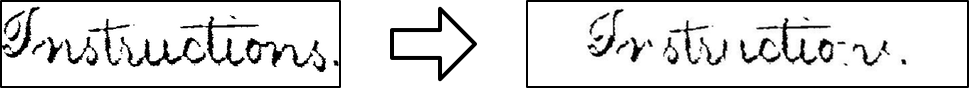
\includegraphics[width=8cm]{damage-simulation}
\end{center}
\caption{An original word image from the George Washington dataset (left), and the same word after applying damage blocks to simulate ink deterioration (right).}
\label{fig:damage-simulation}
\end{figure}


\subsection{Feature Extraction}
Histogram of oriented gradients (HoG) features were used as features for the images. Although more advanced features are available that result in better accuracy, the goal was to apply a proven technique that would provide adequate baseline performance. This portion of the system is modular, so an improved feature extraction system would be straightforward to implement.

HoG features were extracted using a scikit-image implementation \cite{van2014scikit}. The results in this paper were achieved using a HoG descriptor with 9 orientation bins, a cell size of 16pixels x 16pixels, 2x2 cells per block, and L1 normalization.



%
% VAE Details
%
\section{Variational Autoencoder}
\label{sec:vae}

The purpose of the Variational Autoencoder (VAE) \cite{kingma2013auto} in this system is to learn an encoded representation of word images, without the need for ground truth label. After being trained, the VAE can be used to encode word images into features, as well as provide enhancement of damaged words before matching takes place.

The VAE is an unsupervised generative technique. In this case, the VAE works on top of a convolutional neural network and is trained using stochastic gradient descent. As a generative model, its job ``is to somehow capture the dependencies between pixels" \cite{doersch2016tutorial}. After proper training, the VAE should be able to take an input image, create an encoded representation of that image, and then generate a similar image using only the encoding.

For example, an idealized VAE trained on the MNIST dataset would learn an encoding that captured the digits 0 to 9. This encoded layer of the network is referred to as the latent variable, and the latent variables are used to decide which class of output should be generated. If latent variables corresponded to a 1, the decoding portion of the network would generate output that resembled a 1. The structure of the VAE and its overall process is visualized in figure \ref{fig:vaedemo}.

The VAE trains on each dataset separately, so that separate models are created for the George Washington dataset, the Parzival dataset, and the Wycliffe dataset. In the evaluation chapter, these models generate ``restored" versions of the word images before word retrieval takes place, and results are compared to the non-restored word image set.

The VAE was implemented using Keras \cite{chollet2015keras}, with TensorFlow \cite{abadi2016tensorflow} used as the backend.

\subsection{For Feature Extraction}
\textbf{TODO} describe how VAEs can extract features.


\subsection{For Restoration}
\textbf{TODO} describe how VAEs can reconstruct data.


%
% Word retrieval Section (super short?)
%
\section{Word Retrieval}
The current system employs a simple query-by-example method. This means that the query requires a word image as input, rather than a string. Given a word image as input, the query system calculates the HoG feature vector and compares it to the feature vectors for all other word images. The results are sorted by euclidean distance between vectors, and returned in order of proximity.



%
% Data Background Section
%
\section{Providing Labels}
In the experiments, a simulated oracle was used for labeling. Because the word images were sorted in order of appearance in the text, the oracle simply labeled the image using the word at the corresponding index of the transcript. However, this was done purely for evaluation purposes, as one focus of the project was to provide users a way to interact with an automated transcription system.

Users can provide labels to word images in a simple graphical user interface which displays the original word image (before inverting it and removing the background). The interface, built using TKInter, allows a user to type in a label for the word image, skip to the next word, or flag the word image as requiring re-segmentation. The label is stored in a simple file that also records the coordinates of the word and whether segmentation was affirmed.

\subsection{Priority Queue}
The order in which to request labels from users is a key concern. Two simple choices would be in order of appearance, or randomly.

A more useful approach would allow users to label ``interesting'' words. In some cases, that could mean the most frequently occurring words, and in other cases, it could mean labeling the rare words.

(\textbf{TODO} add details about sorting label requests)


%
% Evaluation
%
\section{Evaluation}
Unique metrics are used to objectively evaluate word spotting methods. Most of these metrics are primarily concerned with the {\em precision} of the results. In other words, when a word is queried and the system provides a list of matching word images, the matches are evaluated based on whether those results are correct, and not based on whether it missed other matches in the data.

\subsection{Precision at K}
The precision at k ({\em P@k}) metric is one of the most widely used for evaluating word spotting methods. P@k determines the precision for the {\em k} top retrieved words, or the relevance of the {\em k} top retrieved words.
\begin{center}
\begin{math}
{P@k}=\cfrac{\mid\{relevant\ instances\}\cap\{k\ retrieved\ instances\}\mid} {\mid \{k\ retrieved\ instances\}\mid}
\end{math}
\end{center}

\subsection{Mean Average Precision}
The mean average precision ({\em MAP}) is the most popular evaluation protocol for word spotting. A recent review \cite{giotis2017survey} of nearly 200 papers in word spotting tracked the evaluation metric used in each paper, and conclusively found {\em MAP} to be dominant. The formal definition for {\em Average Precision} is as follows:

\begin{center}
\begin{math}
{AP}=\cfrac{\sum_{k=1}^n (P@k\ \times rel(k))}{\mid\{relevant \ instances\}\mid}
\end{math}
\end{center}

{\em MAP} is the mean value of {\em AP} over all queries. The metric rewards systems that properly sort results according to relevance. If two systems each have three relevant results in the top five matches, they can still produce different scores. Specifically, if one system front-loads the relevant results while the other fails to do so, the former system will produce a better MAP score.


%%
%
%
% Results Chapter
%
%%
\chapter{Results}
The main goal in evaluating the system was to determine whether the VAE could reconstruct damaged words so as to accurately classify them during word spotting.

%
% Data Background Section
%
\section{Datasets}
Three datasets were used to evaluate the interactive approach to word recognition and ink restoration. The first two are benchmark datasets from the literature, and the third is a custom scan of a publicly available document.


\begin{table}[h]
\centering
\begin{tabular}{lllll}
\textbf{Dataset}  & \textbf{Year} & \textbf{Medium}  & \textbf{Words} & \textbf{Unique Words} \\
\hline
George Washington & 1755                  & Ink on paper     & 4,894          & 1,471                 \\
Parzival          & 1200s                 & Ink on parchment & 23,478         & 4,934                 \\
Wycliffe*         & 1388                  & Ink on parchment & 310            & 143                  
\end{tabular}
\caption{Summary table of the datasets used for evaluation. Note the Wycliffe test set is a small subset of the full Wycliffe New Testament.}
\label{table:datasets}
\end{table}

\begin{figure}[t]
\begin{center}
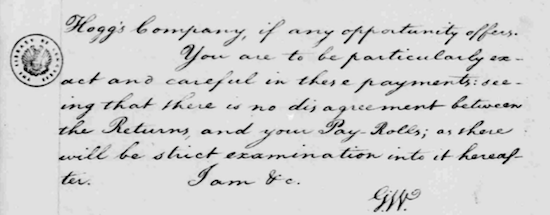
\includegraphics[height=1.8cm]{gw-sample}
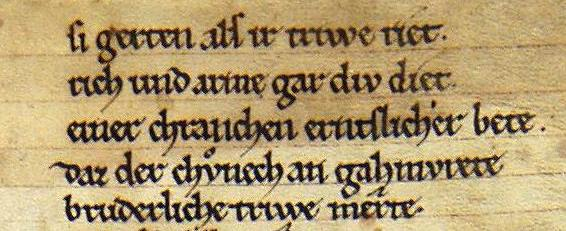
\includegraphics[height=1.8cm]{parzival-sample}
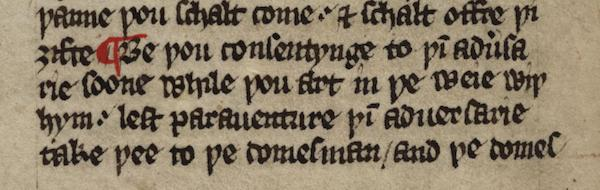
\includegraphics[height=1.8cm]{wycliffe-sample}
\end{center}
\caption{Sample lines from the George Washington dataset (left), the Parzival dataset (middle), and the Wycliffe dataset (right).}
\label{fig:dataset-samples}
\end{figure}


\subsection{George Washington Dataset}
The George Washington Dataset is enormously popular for evaluating handwriting recognition. The subset of data used in this paper is from work done by \cite{fischer2012lexicon}, in which authors provide word segmentation, ground truth, and normalized images for 20 pages of the George Washington letters.

\subsection{Parzival Dataset}
The Parzival database is a medieval German text from the 13th century which was annotated and made publicly available by \cite{fischer2010ground}. It includes nearly 50 manuscript pages. The ink and parchment closely resemble the Wycliffe documents, which is not too surprising given their chronological proximity.

\subsection{Wycliffe Dataset}
The Wycliffe New Testament is a Middle English Bible translation from the 14th century. Numerous copies of Wycliffe's New Testament survive to this day, but the particular manuscript images used in this project were acquired in 2010 from...?


%
% Word Spotting Results
%
\section{Basic Word Spotting}
The goal of the basic word spoting experiments was to determine whether the latent variables in a VAE could adequately serve as features during word spotting. Table \ref{table:word-spotting} shows that VAE-encoded features outperform histograms of oriented gradients, a widely-used feature in word spotting \cite{giotis2017survey}. Word spotting precision at k=5 (P@5) and mean average precision (MAP) are shown in the table.

\begin{table}[h]
\centering
\begin{tabular}{llll}
\textbf{Data}  & \textbf{Feature} & \textbf{P@5} & \textbf{MAP} \\
\hline
Original GW    & HoG			& 0.747          & 0.675          \\
Original GW    & VAE Encoding 	& 0.748          & 0.678          \\
Original Parzival & HoG                     & 0.689          & 0.637          \\
Original Parzival & VAE Encoding 	& 0.771          & 0.720          \\
Original Wycliffe & HoG			& 0.631          & 0.584          \\
Original Wycliffe & VAE Encoding	& 0.768          & 0.662         
\end{tabular}
\caption{Word Spotting Results}
\label{table:word-spotting}
\end{table}




%
% Damaged Data Results
%
\section{Classification on Damaged Datasest}
The goal of experiments on damaged word images was twofold: first, to determine whether VAE features were more suitable for damaged data, and second, to set a baseline performance to be compared against in the following section.

\begin{table}[h]
\centering
\begin{tabular}{llll}
\textbf{Data}  & \textbf{Feature} & \textbf{P@5} & \textbf{MAP} \\
\hline
Damaged GW    & HoG			& 0.602          & 0.547          \\
Damaged GW    & VAE Encoding 	& 0.650          & 0.592          \\
Damaged Parzival & HoG                     & 0.515          & 0.477          \\
Damaged Parzival & VAE Encoding 	& 0.615          & 0.572          \\   
\end{tabular}
\caption{Results for ``Damaged'' Datasets}
\label{my-label}
\end{table}




%
% Reconstructed Data Results
%
\section{Reconstruction Results}
This section evaluated the word spotting system on reconstructed or restored word images. Details on the restorative VAE can be found in section \ref{sec:vae}.

\begin{table}[h]
\centering
\begin{tabular}{llll}
\textbf{Data}  & \textbf{Feature} & \textbf{P@5 (change)} & \textbf{MAP (change)} \\
\hline
Reconstructed GW    & HoG			& 0.644 (+0.0)          & 0.583 (+0.0)         \\
Reconstructed GW    & VAE Encoding 	& 0.665 (+0.0)         & 0.604 (+0.0)         \\
Reconstructed Parzival & HoG                     & 0.554 (+0.0)         & 0.512 (+0.0)         \\
Reconstructed Parzival & VAE Encoding 	& 0.620 (+0.0)         & 0.577 (+0.0)         \\
Reconstructed Wycliffe & HoG                     & 0.873 (+0.0)         & 0.768 (+0.0)         \\
Reconstructed Wycliffe & VAE Encoding 	& 0.859 (+0.0)         & 0.755 (+0.0)         \\
\end{tabular}
\caption{Results for Reconstructed Data}
\label{my-label}
\end{table}





%%
%
%
% Introduction Chapter
%
%%
\chapter{Conclusion}

\section{Challenges}
What I ran into.

\section{Findings}
What I found.

\section{Future Work}
Suggestions for future work.




\copyrightnotice
%-----------------------------------------------
\backmatter
\bibliographystyle{unsrt}   % this means that the order of references
			    % is dtermined by the order in which the
			    % \cite and \nocite commands appear
\bibliography{mybib}  % list here all the bibliographies that
			     % you need. 

\chapter{Vita}
A brief vita goes here.
\end{document}